\chapter{Linear classifiers}
\label{chap-classification}

%%%%%%%%%%%%%%%%%%%%%%%%%%%%%%%%%%%%%%%%%%%%%%%%%%%%%%%%%%%%%%%%%%%%%%%%%%%%%
\section{Classification}

A binary {\em{classifier}} is  \anchorednote{a mapping from $\R^d \rightarrow \{-1, +1\}$.}{Actually,
  general classifiers can have a range which is any discrete set, but we'll
  work with this specific case for a while.}  We'll often use the
letter $h$ (for hypothesis) to stand for a classifier, so
the classification process looks like:
$$ x \rightarrow \boxed{h} \rightarrow y \;\;.$$

Real life rarely gives us vectors of real numbers;  the $x$ we really
want to classify is usually something like  a song, image, or person.
In that case, we'll have to define a function $\varphi(x)$, whose
domain is $\R^d$, where $\varphi$ represents
  {\em features} of $x$, like a person's height or the amount of bass in
a song, and then let the $h: \varphi(x) \rightarrow \{-1, +1\}$.
In much of the following, we'll omit explicit mention of $\varphi$ and
assume that the $\ex{x}{i}$ are in $\R^d$, but you should always have
in mind that some additional process was almost surely required to go
from the actual input examples to their feature representation.

In {\em{supervised learning}} we are given a training data set of the
form
\[ \data_n = \left\{\left(\ex{x}{1}, \ex{y}{1}\right), \dots, \left(\ex{x}{n},
  \ex{y}{n}\right)\right\} \;\;.\]
We will assume that each $\ex{x}{i}$ is a $d \times 1$ {\em column
    vector}. The intended meaning of this data is that, when given an input
$\ex{x}{i}$, the learned hypothesis should generate output
$\ex{y}{i}$.

What makes a classifier useful? That it works well on {\em new} data;
that is, that it makes good predictions on \anchorednote{examples it hasn't
  seen.}{My favorite analogy is to problem sets.  We evaluate a
  student's ability to {\em generalize} by putting questions on
  the exam that were not on the homework (training set).}
But we don't know exactly what data this classifier might be tested on
when we use it in the real world. So, we have to {\em{assume}} a
connection between the training data and testing data; typically, they
are drawn independently from the same probability distribution.

Given a training set $\data_n$ and a classifier $h$, we can define the
  {\em{training error}} of $h$ to be
\begin{eqnarray*}
  \trainerr(h) = \frac{1}{n}\sum_{i = 1}^{n}\begin{cases} 1 &
              h(\ex{x}{i}) \ne \ex{y}{i} \\ 0 & \text{otherwise}\end{cases}
  \;\;.
\end{eqnarray*}

For now, we will try to find a classifier with small training error
(later, with some added criteria) and hope it {\em{generalizes well}}
to new data, and has a small {\em test error}
\begin{eqnarray*}
  \mathcal{E}(h) = \frac{1}{n'}\sum_{i = n + 1}^{n + n'}\begin{cases}
    1 & h(x^{(i)}) \ne y^{(i)} \\ 0 & \text{otherwise}\end{cases}
\end{eqnarray*}
on $n'$ new examples that were not used in the process of finding the
classifier.

%%%%%%%%%%%%%%%%%%%%%%%%%%%%%%%%%%%%%%%%%%%%%%%%%%%%%%%%%%%%%%%%%%%%%%%%%%%%%
\section{Learning algorithm}
A {\em hypothesis class} $\hclass$ is a set (finite or infinite) of
possible classifiers, each of which represents a mapping from
$\R^d \rightarrow \{-1, +1\}$.

A {\em learning algorithm} is a
procedure that takes a data set $\data_n$ as input and returns an
element $h$ of $\hclass$;  it looks  like
\begin{equation*}
  \data_n \longrightarrow \boxed{\text{learning alg ($\hclass$)}} \longrightarrow h
\end{equation*}

We will find that the choice of $\hclass$ can have a big impact on the
test error of the $h$ that results from this process.
One way to get $h$ that generalizes well is to restrict the size, or
``expressiveness'' of $\hclass$.

%%%%%%%%%%%%%%%%%%%%%%%%%%%%%%%%%%%%%%%%%%%%%%%%%%%%%%%%%%%%%%%%%%%%%%%%%%%%%
\section{Linear classifiers}

We'll start with the hypothesis class of {\em linear classifiers}.
They are (relatively) easy to understand, simple in a mathematical
sense, powerful on their own, and the basis for many other more
sophisticated methods.

A linear classifier in $d$ dimensions is
defined by a vector of parameters $\theta \in \R^d$ and scalar
$\theta_0 \in \R$.  So, the hypothesis class $\hclass$ of linear
classifiers in $d$ dimensions is the {\em set} of all vectors in
$\R^{d+1}$.   We'll assume that $\theta$ is a $d \times 1$ column
vector.

Given particular values for $\theta$ and $\theta_0$, the  \anchorednote{classifier is
  defined by}{Let's be careful about dimensions.  We have assumed that $x$ and
  $\theta$ are both $d \times 1$ column vectors.  So $\theta^T x$ is $1
    \times 1$, which in math (but not necessarily numpy) is the same as a
  scalar.}
\begin{eqnarray*}
  h(x; \theta, \theta_0) = \text{sign}(\theta^T x + \theta_0)
  = \begin{cases} +1 & \text{if $\theta^Tx + \theta_0 > 0$} \\ -1 &
              \text{otherwise}\end{cases} \;\;.
\end{eqnarray*}
Remember that we can think of $\theta, \theta_0$ as specifying a
hyperplane.  It divides $\R^d$, the space our $\ex{x}{i}$ points live
in, into two half-spaces.  The one that is on the same side as the
normal vector is the {\em positive} half-space, and we classify all
points in that space as positive.  The half-space on the other side is
  {\em negative} and all points in it are classified as negative.

\begin{examplebox}{\bf Example:}
  Let $h$ be the linear classifier defined by
  $\theta = \protect\twodcol{-1}{1.5}, \theta_0 = 3$.

  \noindent The diagram below shows several points classified by $h$.
  In particular, let $\ex{x}{1} = \twodcol{3}{2}$ and
  $\ex{x}{2} = \twodcol{4}{-1}$.
  \begin{align*}
    h(\ex{x}{1}; \theta, \theta_0) & = \sign\left(\twodrow{-1}{1.5}\twodcol{3}{2} + 3\right) = \sign(3) = +1     \\
    h(\ex{x}{2}; \theta, \theta_0) & = \sign\left(\twodrow{-1}{1.5}\twodcol{4}{-1} + 3\right) = \sign(-2.5) = -1
  \end{align*}
  Thus, $\ex{x}{1}$ and $\ex{x}{2}$ are given positive and negative classfications,
  respectively.

  \begin{tikzpicture}
    \draw [thin, gray!40] (-2,-3) grid (5,4);
    \draw [<->] (-2,0) -- (5,0);
    \draw [<->] (0,-3) -- (0,4);

    \draw [ultra thick] (-1.5,-3) -- (5,1.3333)
    node [above right] {\large$\theta^Tx + \theta_0 = 0$};

    \draw [thick,teal,-latex] (2,-0.6667) -- (1,0.8883)
    node [black,below left] {$\theta$};

    \node [above right,xshift=.3em] at (3,2) {\large$\ex{x}{1}$};
    \node [above right,xshift=.3em] at (4,-1) {\large$\ex{x}{2}$};


    \foreach \Point in {(3,2), (1.8,3.5), (-1,3), (.8,-.6), (-1.4,-.9),
        (1.5, 1.5)}{
        \pic at \Point {plus};
      }

    \foreach \Point in {(4,-1), (2,-2.7), (4.4,-2.1)}{
        \pic at \Point {minus};
      }
  \end{tikzpicture}

\end{examplebox}

\question{What is the green vector normal to the hyperplane?  Specify it
  as a column vector.}
\question{
  What change would you have to make to $\theta, \theta_0$ if you wanted
  to have the separating hyperplane in the same place, but to classify
  all the points labeled '+' in the diagram as negative and all the
  points labeled '-' in the diagram as positive?}

%%%%%%%%%%%%%%%%%%%%%%%%%%%%%%%%%%%%%%%%%%%%%%%%%%%%%%%%%%%%%%%%%%%%%%%%%%%%%
\section{Learning linear classifiers}

Now, given a data set and the hypothesis class of linear classifiers,
our objective will be to find the linear classifier with the smallest
possible training error.
  %This strategy is (mostly) okay because the
  %class of linear classifiers is, in some sense, small.

  {\em This is a well-formed optimization problem. But it's not
    computationally easy!}

We'll start by considering a very simple learning algorithm. \note{It's
  a good idea to think of the ``stupidest possible'' solution to a
  problem, before trying to get clever.  Here's a fairly (but not
  completely) stupid algorithm.}  The idea is to generate $k$ possible
hypotheses by generating their parameter vectors at random.  Then, we
can evaluate the training-set error on each of the hypotheses and
return the hypothesis that has the lowest training error (breaking
ties arbitrarily).

\begin{codebox}
  \Procname{$\proc{Random-Linear-Classifier}(\dataTrain, k)$}
  \li \For $j \gets 1$ \To $k$
  \li   \Do
  randomly sample $\left(\ex{\theta}{j},
    \ex{\theta_0}{j}\right)$ from $(\R^d, \R)$
  \End
  \li $j^* \gets \argmin{j \in \{1, \ldots, k\}} \mathcal{E}_n \left(\ex{\theta}{j}, \ex{\theta_0}{j}\right)$
  \li \Return $\left(\ex{\theta}{j^*}, \ex{\theta_0}{j^*}\right)$
\end{codebox}



A note about terminology and
\anchorednote{notation.}
{The notation within the algorithm above might be new to you:
  $\argmin{x} f(x)$
  means the value of $x$ for which $f(x)$ is the smallest.  Sometimes
  we write $\argmin{x \in {\cal X}} f(x)$ when we want to explicitly
  specify the set ${\cal X}$ of values of $x$ over which we want to
  minimize.}
The training data $\dataTrain$ is an input to the learning algorithm,
and the output of this learning algorithm will be a hypothesis $h$, where
$h$ has parameters $\theta$ and $\theta_{0}.$
In contrast to $\theta$ and $\theta_{0}$, the input $k$ is a
parameter of the learning algorithm itself; such
parameters are often called {\em hyperparameters}.

\question{
  What do you think will be observed for $\trainerr(h)$, where $h$ is the
  hypothesis returned by \proc{Random-Linear-Classifier}, if this learning
  algorithm is run multiple times? And as $k$ is increased? }

\question{
  What properties of $\dataTrain$ do you think will have an
  effect on $\trainerr(h)$?
}

%%%%%%%%%%%%%%%%%%%%%%%%%%%%%%%%%%%%%%%%%%%%%%%%%%%%%%%%%%%%%%%%%%%%%%%%%%%%%
\section{Evaluating a learning algorithm}
How should we evaluate the performance of a {\em classifier} $h$?   The best
method is to measure {\em test error} on data that was not used to
train it.

How should we evaluate the performance of a {\em learning algorithm}?
This is trickier.  There are many potential sources of variability in
the possible result of computing test error on a learned hypothesis $h$:
\begin{itemize}
  \item Which particular {\em training examples} occurred in $\dataTrain$
  \item Which particular {\em testing examples} occurred in $\dataTest$
  \item Randomization inside the learning {\em algorithm} itself
\end{itemize}
Generally, we would like to execute the following process multiple
times:
\begin{itemize}
  \item Train on a new training set
  \item Evaluate resulting $h$ on a testing set {\em that does not
            overlap the training set}
\end{itemize}
Doing this multiple times controls for possible poor choices of
training set or unfortunate randomization inside the algorithm itself.

One concern is that we might need a lot of data to do this, and in
many applications data is expensive or difficult to acquire. We can
re-use data with {\em{cross validation}} (but it's harder to do theoretical
analysis).  \\
\begin{codebox}
  \Procname{$\proc{Cross-Validate}(\data, k)$}
  \li divide $\data$ into $k$ chunks $\data_1, \data_2, \ldots \data_k$ (of roughly equal size)
  \li \For $i \gets 1$ \To $k$
  \li   \Do
  train $h_i$ on $\data \setminus \data_i$ (withholding chunk $\data_i$)
  \li     compute ``test'' error $\mathcal{E}_i (h_i)$ on withheld data $\data_i$
  \End
  \li \Return $\frac{1}{k} \sum_{i=1}^k \mathcal{E}_i (h_i)$
\end{codebox}

It's very important to understand that cross-validation neither
delivers nor evaluates a single particular hypothesis $h$.  It
evaluates the {\em algorithm} that produces hypotheses.

%%%%%%%%%%%%%%%%%%%%%%%%%%%%%%%%%%%%%%%%%%%%%%%%%%%%%%%%%%%%%%%%%%%%%%%%%%%%%
\section{Feature representation for classifiers}

Linear classifiers are easy to work with and analyze, but they are a
very restricted class of hypotheses.  If we have to make a complex
distinction in low dimensions, then they are unhelpful.

Our favorite illustrative example is the ``exclusive or'' ({\sc xor})
data set, the drosophila \note{D. Melanogaster is a species of fruit
  fly, used as a simple system in which to study genetics, since 1910.}
of machine-learning data sets:

\begin{examplebox}
  \begin{center}
    \begin{tikzpicture}
      \pic at (-1, -1) {plusblk};
      \pic at (-1, +1) {minusblk};
      \pic at (+1, -1) {minusblk};
      \pic at (+1, +1) {plusblk};
    \end{tikzpicture}
  \end{center}
\end{examplebox}

There is no linear separator for this two-dimensional dataset!  But, we have a trick
available:  take a low-dimensional data set and move it, using a
non-linear transformation into a higher-dimensional space, and look
for a linear separator there. Let's look at an example data set that
starts in 1-D:

\begin{examplebox}
  \begin{center}
    \begin{tikzpicture}
      \draw [<->, gray] (-3,0) -- (3,0)
      node [black, right] {$x$};
      \draw [gray] (0,.6) -- (0,-.6)
      node [black, below] {0};

      \pic at (-1.5, 0) {plusblk};
      \pic at (-.5, 0) {minusblk};
      \pic at (.5, 0) {minusblk};
      \pic at (1.5, 0) {plusblk};

    \end{tikzpicture}
  \end{center}
\end{examplebox}

These points are not linearly separable, \note{What's a linear
  separator for data in 1D?  A point!}  but consider the
transformation $\phi(x) = [x,x^2]$. Putting the data in $\phi$ space,
we see that it is now separable.  There are lots of possible
separators;  we have just shown one of them here.

\begin{examplebox}
  \begin{center}
    \begin{tikzpicture}
      \draw [<->, gray] (-3,0) -- (3,0)
      node [black, right] {$x$};
      \draw [<->, gray] (0,-.6) -- (0,4)
      node [black, above] {$x^2$};

      \draw [dashed] (-3, 1.25) -- (3, 1.25)
      node [below, xshift=-1cm] {separator};

      \pic at (-1.5, 2.25) {plusblk};
      \pic at (-.5, .25) {minusblk};
      \pic at (.5, .25) {minusblk};
      \pic at (1.5, 2.25) {plusblk};

    \end{tikzpicture}
  \end{center}
\end{examplebox}

A linear separator in $\phi$ space is a nonlinear separator in the
original space!  Let's see how this plays out in our simple example.
Consider the separator $x^2  - 1 = 0$, which labels the half-plane
$x^2 -1 > 0$ as positive.  What separator does it correspond to in the
original 1-D space?
We have to ask the question:  which $x$ values have the property that
$x^2 - 1 = 0$.  The answer is $+1$ and $-1$, so those two points
constitute our separator, back in the original space.  And we can use
the same reasoning to find the region of 1D space that is labeled
positive by this separator.

\begin{examplebox}
  \begin{center}
    \begin{tikzpicture}
      \draw [<->, gray] (-3,0) -- (3,0)
      node [black, right] {$x$};
      \draw [gray] (0,.6) -- (0,-.6)
      node [black, below] {0};
      \draw [gray] (1,.2) -- (1,-.2)
      node [black, below] {1};
      \draw [gray] (-1,.2) -- (-1,-.2)
      node [black, below] {-1};

      \fill (1,0) circle (2.5pt);
      \fill (-1,0) circle (2.5pt);

      \draw[decoration={calligraphic brace,amplitude=5pt}, decorate, line width=1.25pt]
      (-2.95,0.2) node {} -- (-1.05,0.2);
      \draw[decoration={calligraphic brace,amplitude=5pt}, decorate, line width=1.25pt]
      (-.95,0.2) node {} -- (.95,0.2);
      \draw[decoration={calligraphic brace,amplitude=5pt}, decorate, line width=1.25pt]
      (1.05,0.2) node {} -- (2.95,0.2);

      \pic at (-2, 0.7) {plus};
      \pic at (0, 0.7) {minus};
      \pic at (2, 0.7) {plus};

    \end{tikzpicture}
  \end{center}
\end{examplebox}

This is a very general and widely useful strategy.  It's the basis for
  {\em kernel methods}, a powerful technique that we unfortunately won't
get to in this class, and can be seen as a motivation for multi-layer
neural networks.

%%%%%%%%%%%%%%%%%%%%%%%%%%%%%%%%%%%%%%%%
\subsection{Feature representation for XOR}

% FIXME: regenerate plots using optimization algorithm instead of perceptron

So, what if we try to solve the {\sc xor} problem using a polynomial
basis as the feature transformation?  We can just take our
two-dimensional data and transform it into a higher-dimensional data
set, by applying $\phi$.  Now, we have a classification problem as
usual, and we can use the perceptron algorithm to solve it.

Let's try it for $k = 2$ on our {\sc xor} problem.  The feature
transformation is
\[\phi((x_1, x_2)) = (1, x_1, x_2, x_1^2, x_1 x_2, x_2^2)\;\;.\]
\question{
  If we train a classifier after performing this feature
  transformation, would we lose any expressive
  power if we let $\theta_0 = 0$ (i.e. trained without offset instead of
  with offset)?}
After several iterations, we find a separator
with coefficients $\theta = (0, 0, 0, 0, 4, 0)$ and $\theta_0 =
  0$.
This corresponds to
\[0 + 0 x_1 + 0 x_2 + 0 x_1^2 + 4 x_1 x_2 + 0x_2^2 + 0 = 0\]
and is plotted below, with the gray shaded region classified as
negative and the white region classified as positive:
\begin{examplebox}
  \begin{center}
    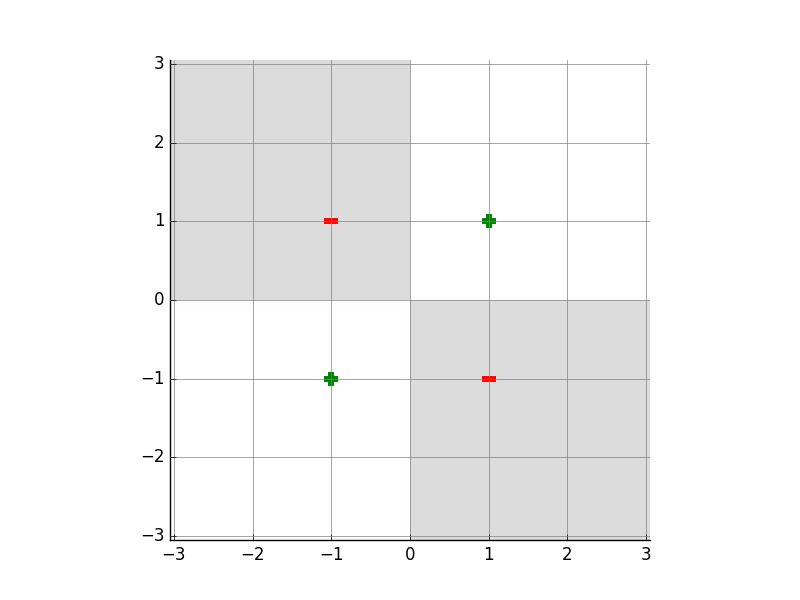
\includegraphics[scale=0.3]{figures/feature_representation_1.png}
  \end{center}
\end{examplebox}
\question{
  Be sure you understand why this high-dimensional hyperplane is a
  separator, and how it corresponds to the figure.}

For fun, we show some more plots below.  Here is the result of generating a linear classifier
on {\sc xor}, but where the data are put in a different
place on the plane: %  After 65 mistakes (!) it arrives at these coefficients:
$\theta = ( 1, -1, -1, -5, 11, -5)$, $\theta_0 =  1$, which generates
this separator:
\note{The jaggedness
  in the plotting of the separator is an artifact of a lazy lpk strategy
  for making these plots--the true curves are smooth.
}
\begin{examplebox}
  \begin{center}
    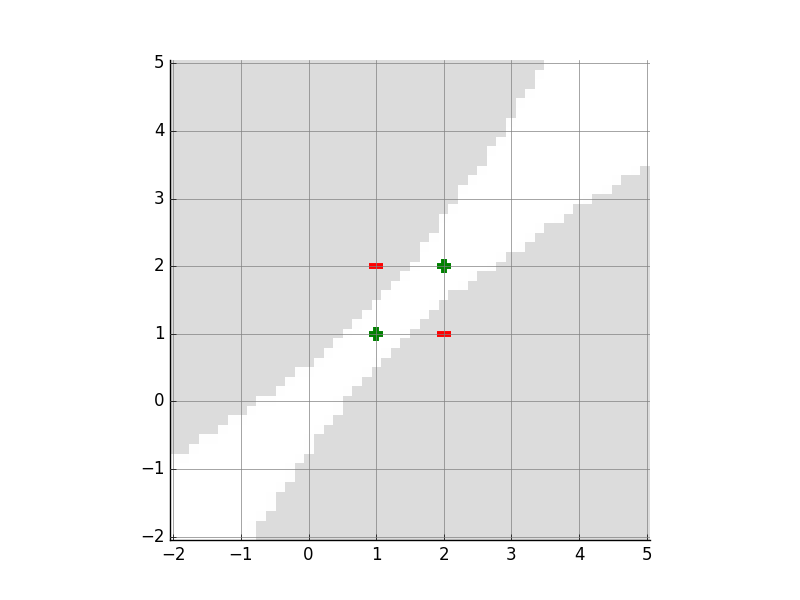
\includegraphics[scale=0.3]{figures/feature_representation_2.png}
  \end{center}
\end{examplebox}
\question{It takes many more iterations to solve this
  version.  Apply knowledge of the convergence properties of the
  perceptron to understand why.}

Here is a harder data set.  After 200 iterations, we could not		% FIXME: iterations of what?
separate it with a second or third-order basis representation.  Shown
below are the results after 200 iterations for bases of order 2, 3, 4,
and 5.
\begin{examplebox}
  \begin{center}
    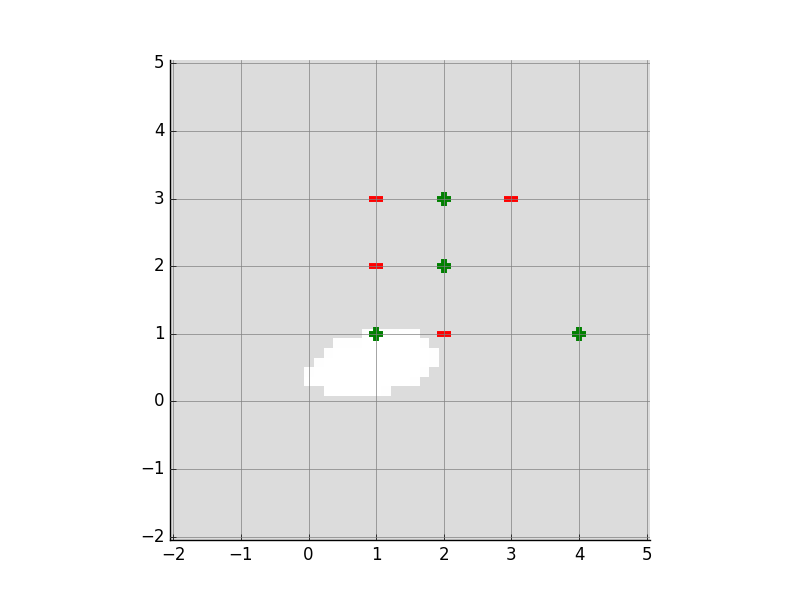
\includegraphics[width=0.48\linewidth]{figures/feature_representation_3.png}
    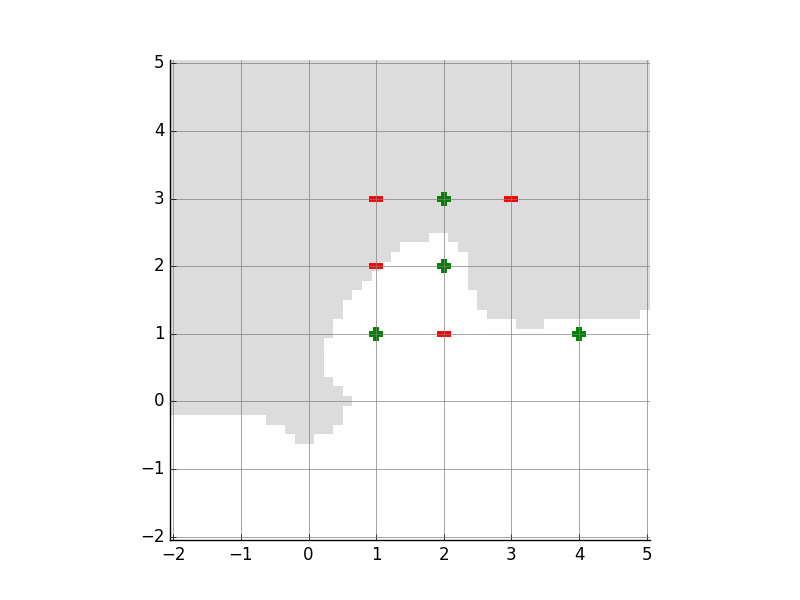
\includegraphics[width=0.48\linewidth]{figures/feature_representation_4.png} \\
    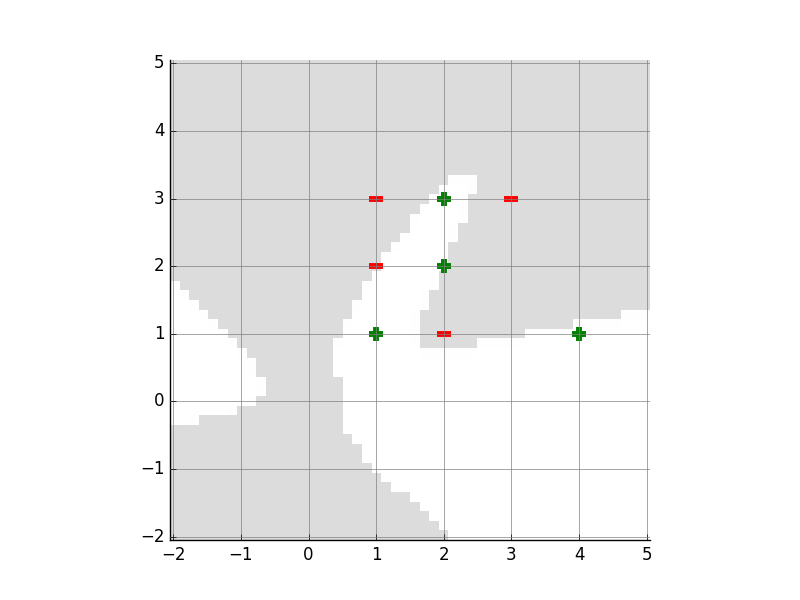
\includegraphics[width=0.48\linewidth]{figures/feature_representation_5.png}
    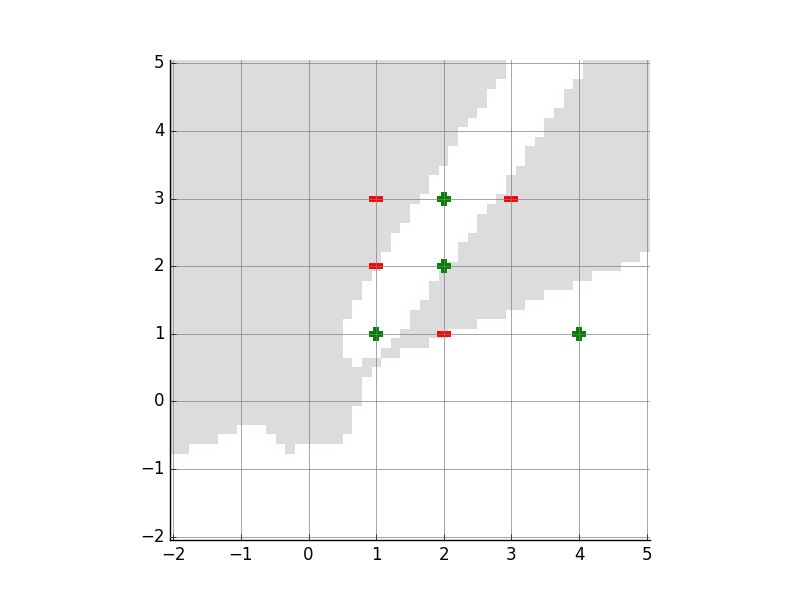
\includegraphics[width=0.48\linewidth]{figures/feature_representation_6.png}
  \end{center}
\end{examplebox}


%%% Local Variables:
%%% mode: latex
%%% TeX-master: "top"
%%% End:
